\documentclass[preview]{standalone}

\usepackage{amsmath}
\usepackage{amssymb}
\usepackage{stellar}
\usepackage{definitions}
\usepackage{tikz}
\usepackage{pgfplots}

\usetikzlibrary{3d, decorations.markings, calc, perspective, shadings, calc, arrows.meta}
\pgfplotsset{compat=1.18}

\tikzset{
    labelstyle/.style={align=center, font=\Large, gray!80!black},
    mathstyle/.style={font=\sffamily\Large\bfseries},
    arrowstyle/.style={->, -Latex, thick, gray!60, shorten >= 3pt, shorten <= 3pt},
    boundarythick/.style={line width=1.5pt}
}

\begin{document}

\id{topology-constructions}
\genpage

\section{Spheres and disks}

\begin{snippetdefinition}{disk-definition}{Disk}
    The \emph{disk} is defined as
    \[
        D^n = \{
            x \in \realnumbers^n
            \suchthat ||x|| \leq 1
        \}
    \]
\end{snippetdefinition}

\begin{snippetdefinition}{sphere-definition}{Sphere}
    The \emph{sphere} is defined as
    \[
        S^n = \{
            x \in \realnumbers^{n+1}
            \suchthat ||x|| = 1
        \}
    \]
\end{snippetdefinition}

\begin{snippettheorem}{sphere-disk-relation-theorem}{}
    \[ % TODOURGENT homeomorphic
        \boundary[\realnumbers^n][D^n] \cong S^{n-1}
    \]
\end{snippettheorem}

\begin{snippet}{sphere-disk-illustration}
    \begin{center}
        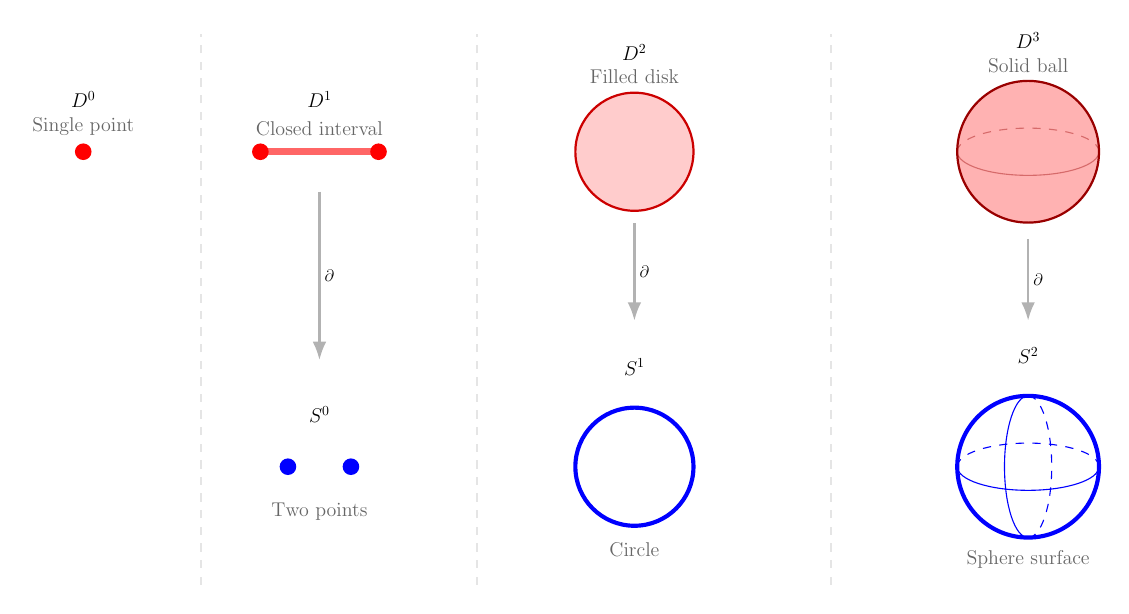
\begin{tikzpicture}[scale=0.5, transform shape, >=Latex]

        \def\toprowy{8cm} 
        \def\bottomrowy{0cm}

        % ================= COLUMN 0: D^0 =================
        \begin{scope}[xshift=0cm]
            % D^0
            \begin{scope}[yshift=\toprowy]
                \fill[red] (0,0) circle (6pt);
                \node[mathstyle, above=1cm] at (0,0) {$D^0$};
                \node[labelstyle, above=0.3cm] at (0,0) {Single point};
            \end{scope}
        \end{scope}

        % ================= COLUMN 1: D^1 and S^0 =================
        \begin{scope}[xshift=6cm]
            % D^1
            \begin{scope}[yshift=\toprowy]
                \draw[line width=2.5pt, red!60] (-1.5,0) -- (1.5,0);
                \fill[red] (-1.5,0) circle (6pt);
                \fill[red] (1.5,0) circle (6pt);
                
                \node[mathstyle, above=1cm] at (0,0) {$D^1$};
                \node[labelstyle, above=0.3cm] at (0,0) {Closed interval};
                
                % Boundary Arrow
                \draw[arrowstyle] (0,-0.8) -- (0,-5.5) node[midway, right, font=\large, black] {$\partial$};
            \end{scope}
            
            % S^0
            \begin{scope}[yshift=\bottomrowy]
                \fill[blue] (-0.8,0) circle (6pt);
                \fill[blue] (0.8,0) circle (6pt);
                \node[mathstyle, above=1cm] at (0,0) {$S^0$};
                \node[labelstyle, below=0.8cm] at (0,0) {Two points};
            \end{scope}
        \end{scope}

        % ================= COLUMN 2: D^2 and S^1 =================
        \begin{scope}[xshift=14cm]
            % D^2
            \begin{scope}[yshift=\toprowy]
                \filldraw[fill=red!20, draw=red!80!black, thick] (0,0) circle (1.5cm);
                
                \node[mathstyle, above=2.2cm] at (0,0) {$D^2$};
                \node[labelstyle, above=1.6cm] at (0,0) {Filled disk};
                
                % Boundary Arrow
                \draw[arrowstyle] (0,-1.6) -- (0,-4.5) node[midway, right, font=\large, black] {$\partial$};
            \end{scope}

            % S^1
            \begin{scope}[yshift=\bottomrowy]
                \draw[boundarythick, blue] (0,0) circle (1.5cm);
                \node[mathstyle, above=2.2cm] at (0,0) {$S^1$};
                \node[labelstyle, below=1.8cm] at (0,0) {Circle};
            \end{scope}
        \end{scope}

        % ================= COLUMN 3: D^3 and S^2 =================
        \begin{scope}[xshift=24cm]
            % D^3
            \begin{scope}[yshift=\toprowy]
                \fill[red!30] (0,0) circle (1.8cm);
                \draw[red!60!black, thick] (0,0) circle (1.8cm);
                
                % 3D Lines
                \draw[red!60!black, thin, opacity=0.4] (-1.8,0) arc (180:360:1.8cm and 0.6cm);
                \draw[red!60!black, thin, dashed, opacity=0.4] (1.8,0) arc (0:180:1.8cm and 0.6cm);
                
                \node[mathstyle, above=2.5cm] at (0,0) {$D^3$};
                \node[labelstyle, above=1.9cm] at (0,0) {Solid ball};
                
                % Boundary Arrow
                \draw[arrowstyle] (0,-2.0) -- (0,-4.5) node[midway, right, font=\large, black] {$\partial$};
            \end{scope}

            % S^2
            \begin{scope}[yshift=\bottomrowy]
                \draw[boundarythick, blue] (0,0) circle (1.8cm);
                \draw[blue, thin] (-1.8,0) arc (180:360:1.8cm and 0.6cm);
                \draw[blue, thin, dashed] (1.8,0) arc (0:180:1.8cm and 0.6cm);
                \draw[blue, thin] (0,1.8) arc (90:270:0.6cm and 1.8cm);
                \draw[blue, thin, dashed] (0,-1.8) arc (-90:90:0.6cm and 1.8cm);
                
                \node[mathstyle, above=2.5cm] at (0,0) {$S^2$};
                \node[labelstyle, below=2.0cm] at (0,0) {Sphere surface};
            \end{scope}
        \end{scope}

        % --- Separators ---
        \draw[gray!20, dashed, thick] (3, -3) -- (3, 11);
        \draw[gray!20, dashed, thick] (10, -3) -- (10, 11);
        \draw[gray!20, dashed, thick] (19, -3) -- (19, 11);

        \end{tikzpicture}
    \end{center}
\end{snippet}

\section{Gluing}

\begin{snippetdefinition}{mobius-strip-definition}{Möbius strip}
    Let \(I = [0,1]\) be the closed unit interval.
    Define the equivalence relation \(\sim\) on \(I\) generated
    by \((0,t) \sim (1,1-t)\).
    The \emph{Möbius strip} is defined as \(M = (I \times I)/\sim\).
\end{snippetdefinition}

\begin{snippet}{mobius-strip-illustration-gluing}
    \begin{center}
        % https://tex.stackexchange.com/questions/118563/moebius-strip-using-tikz
        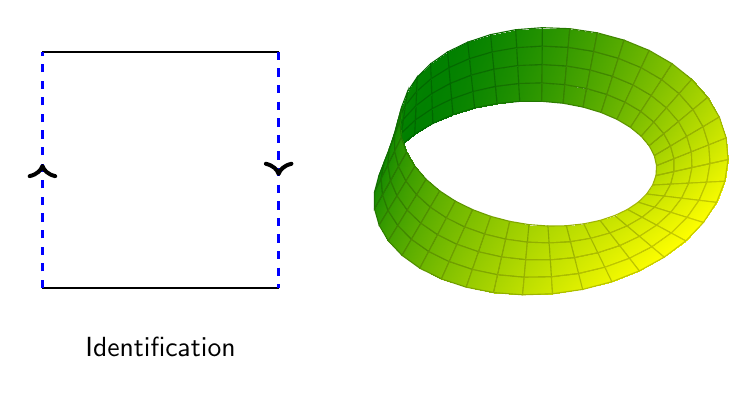
\begin{tikzpicture}
            \tikzset{
                simple mid arrow/.style={
                    postaction={
                        decorate,
                        decoration={
                            markings,
                            mark=at position 0.525 with {\arrow[black, scale=1.2, -{Triangle}]{>}}
                        }
                    }
                }
            }

            \begin{scope}[xshift=-6.5cm, yshift=1cm]
                \coordinate (BL) at (0,0);
                \coordinate (BR) at (3,0);
                \coordinate (TR) at (3,3);
                \coordinate (TL) at (0,3);
                \draw[thick] (BL) -- (BR);
                \draw[thick] (TL) -- (TR);
                \draw[very thick, dashed, blue, simple mid arrow] (BL) -- (TL);
                \draw[very thick, dashed, blue, simple mid arrow] (TR) -- (BR);
                \node[below=0.5cm, font=\sffamily] at (1.5,0) {Identification};
            \end{scope}

            \begin{axis}[
                yshift=2.5cm,
                anchor=center, % Anchor at the center of the plot
                hide axis,
                view={40}{40},
                width=8cm, height=8cm,
                axis equal,
                /tikz/background rectangle/.style={fill=none}
            ]
                % The Surface
                \addplot3 [
                    surf,
                    shader=faceted interp,
                    point meta=x,
                    colormap/greenyellow,
                    samples=40,
                    samples y=5,
                    z buffer=sort,
                    domain=0:360,
                    y domain=-0.5:0.5,
                    thin
                ] (
                    {(1+0.5*y*cos(x/2))*cos(x)},
                    {(1+0.5*y*cos(x/2))*sin(x)},
                    {0.5*y*sin(x/2)}
                );
            \end{axis}

        \end{tikzpicture}
    \end{center}
\end{snippet}

\begin{snippetdefinition}{klein-bottle-definition}{Klein's bottle}
    Let \(I = [0,1]\) be the closed unit interval.
    Define the equivalence relation \(\sim\) on \(I\) generated
    by \((x,0) \sim (x,1)\) and \((0,y) \sim (1,1-y)\).
    The \emph{Klein's bottle} is defined as \(K = (I \times I)/\sim\).
\end{snippetdefinition}

\end{document}